\section{Varias vidas}
\label{sec:varias-vidas}
\newcommand{\NInicialB}{104\,004}
\newcommand{\NMenoresB}{6\,755}
\newcommand{\NParejasTeoricasB}{97\,249}
\newcommand{\NExcluidasB}{0}
\newcommand{\NParejasB}{97\,249}
\newcommand{\VPambosB}{407\,048,93}
\newcommand{\VPultimoB}{431\,032,88}
\newcommand{\VPreversionB}{11\,555,86}
\newcommand{\DiferenciaVPultimoB}{23\,983,95}
\newcommand{\AumentoVPultimoB}{5,89}
\newcommand{\VPreversionHombresB}{7\,767,88}
\newcommand{\VPreversionMujeresB}{3\,787,98}


\textbf{Población y parejas.} Partimos de los \NInicialB{} activos depurados de A.
Los \NMenoresB{} menores de 30 años no generan pagos en B. Los restantes
\NParejasTeoricasB{} reciben una pareja hipotética de sexo opuesto, sin emparejar
registros del Excel. Si el activo es hombre, $y=x-\delta(x)$; si es mujer,
$y=x+\delta(x)$, con $\delta=0$ para $30\leq x<35$, $3$ para $35\leq x<55$
y $5$ para $x\geq55$. Por ejemplo, un hombre de 45 años recibe una pareja mujer
de 42 y una mujer de 45 recibe una pareja hombre de 48. La asignación se fija
al inicio y ambas edades aumentan una unidad por año.

Se verificó que la edad inicial del cónyuge no excediera 106 y que existieran
los cinco $q$ anuales de ambas vidas. Las exclusiones propias de B fueron
\NExcluidasB{}, por lo que se valoraron \NParejasB{} parejas.

\textbf{Supervivencia y rentas.} B utiliza exclusivamente mortalidad biológica,
sin renuncia. Para la cohorte inicial $(x,s)$ y su pareja $(y,s^*)$, definimos
\[
 S_x(t)=\prod_{j=0}^{t-1}(1-q_{x+j,s}),\qquad
 S_y(t)=\prod_{j=0}^{t-1}(1-q_{y+j,s^*}),\quad t=1,\ldots,5.
\]
Bajo independencia entre los tiempos de vida, las probabilidades al cierre son
\[
 \begin{aligned}
 J_t&=S_x(t)S_y(t) &&\text{(ambos vivos)},\\
 U_t&=S_x(t)+S_y(t)-S_x(t)S_y(t) &&\text{(al menos uno vivo)},\\
 R_t&=S_y(t)[1-S_x(t)] &&\text{(cónyuge vivo con activo fallecido)}.
 \end{aligned}
\]
Cada cobertura paga una unidad al cierre de cada año en que se cumple su
estatus. Con descuento efectivo del $4\%$, su valor agregado es
\[
 VP_h=\sum_{(x,s)\text{ estatus}}n_{x,s}
       \sum_{t=1}^{5}\frac{P_h(x,s;t)}{(1{,}04)^t},
 \qquad h\in\{J,U,R\}.
\]
La ponderación utiliza cantidades \emph{iniciales}; aplicar nuevamente la
población proyectada con renuncias de A reduciría indebidamente estos pagos.

\textbf{Interpretación.} La renta de último sobreviviente presenta el mayor
VP (\VPultimoB{}), porque paga mientras viva cualquiera de las dos personas,
incluso si ambas siguen vivas. La renta conjunta (\VPambosB{}) deja de pagar
cuando fallece la primera. La renta de reversión (\VPreversionB{}) paga solo
cuando el activo ya falleció y su cónyuge sigue vivo; puede pagar en varios
cierres y no es un beneficio único por fallecimiento durante el año.
Los tres VP corresponden a alternativas distintas y no se suman entre sí ni
a los flujos del seguro de C. 
\par
Por ejemplo, si la aseguradora ofreciera una renta anual de 
\$500 USD por pareja, el valor presente esperado de las 
obligaciones se obtendría multiplicando cada VP unitario por 
dicho importe. En este caso, la cobertura de último 
sobreviviente representaría una obligación de \$215\,516\,440, 
mientras que las rentas de vida conjunta y de reversión 
representarían \$203\,524\,465 y \$5\,777\,930, respectivamente.

Estos importes representan el valor al 31/12/2025 de los pagos 
futuros esperados durante los cinco años de cobertura, bajo 
los supuestos de mortalidad y descuento establecidos. De esta 
forma, para un mismo importe anual de renta y una misma 
población, la condición que determina la continuidad de los 
pagos tiene un efecto directo sobre el costo esperado de 
cada alternativa para la aseguradora.

Las cantidades iniciales se toman de las cohortes entregadas en A. El anexo B
presenta los cuadros resumen de población, parejas, probabilidades y VP.
El detalle por cohorte, sexo y año se conserva en los CSV generados.

\begin{figure}[H]
\centering
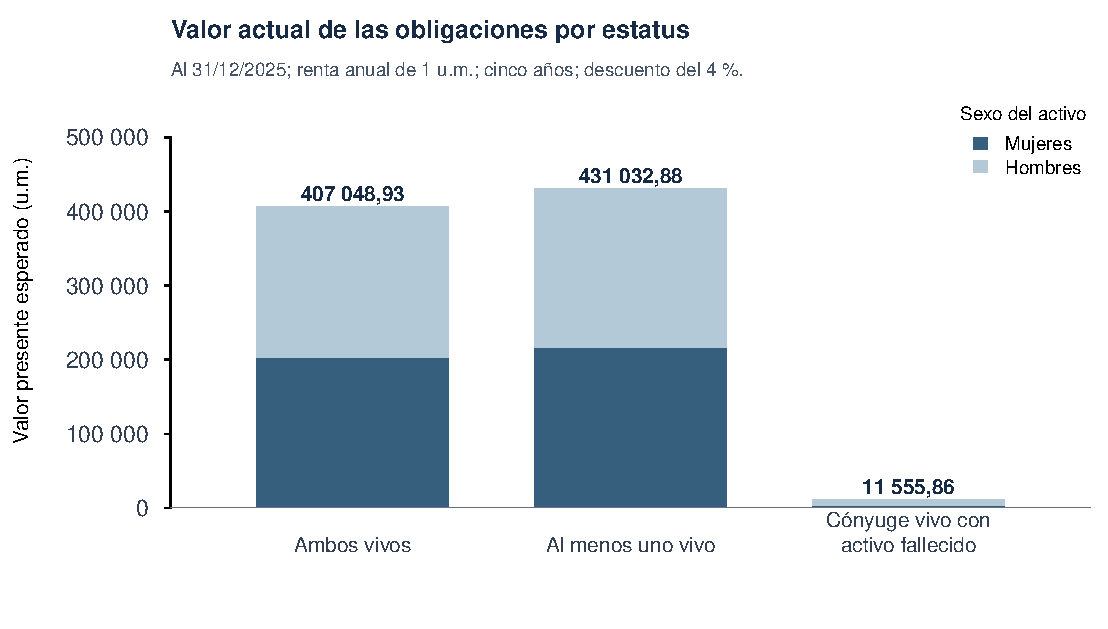
\includegraphics[width=0.96\textwidth]{figuras/vp_varias_vidas.pdf}
\caption{Valor presente esperado al 31/12/2025 de cada renta, desglosado por sexo del activo.
Importes en unidades monetarias para un pago anual de 1 u.m. por pareja.
Elaboración propia.}
\label{fig:vp-varias-vidas}
\end{figure}

Como se observa en el gráfico, la renta de último sobreviviente presenta el mayor valor presente esperado, con 431 032,88 u.m., frente a 407 048,93 u.m. de la renta de ambos vivos. La diferencia es de \DiferenciaVPultimoB{} u.m. (\AumentoVPultimoB{}\%), lo cual se explica porque la primera cobertura mantiene los pagos mientras al menos uno de los integrantes de la pareja continúe con vida.

Por su parte, la renta de reversión presenta un valor considerablemente menor, de 11 555,86 u.m., ya que solo genera pagos cuando el activo ha fallecido y su cónyuge permanece con vida. Dentro de esta cobertura, los activos hombres concentran \VPreversionHombresB{} u.m., frente a \VPreversionMujeresB{} u.m. de las mujeres, diferencia que también está relacionada con las edades y las características de las parejas hipotéticas asignadas.

Estos valores representan los pagos futuros esperados, descontados al inicio de la proyección, para una renta anual de 1 u.m. durante cinco años. 
